\section{Lab2: Osciloscopio y FFT}
%*********************
\begin{frame}{}

\pgfdeclareimage[width=\paperwidth,height=\paperheight]{bg}{imagenes/fondocap2}
\setbeamertemplate{background}{\pgfuseimage{bg}}

\bfseries{\textrm{\LARGE Lab2\\ \Large Osciloscopio y FFT}}
\raggedright
\end{frame}
%*********************

\begin{frame}{Osciloscopio y FFT\index{TCP}}

\pgfdeclareimage[width=\paperwidth,height=\paperheight]{bg}{imagenes/fondo3}
\setbeamertemplate{background}{\pgfuseimage{bg}}

\begin{figure}[H]
\centering
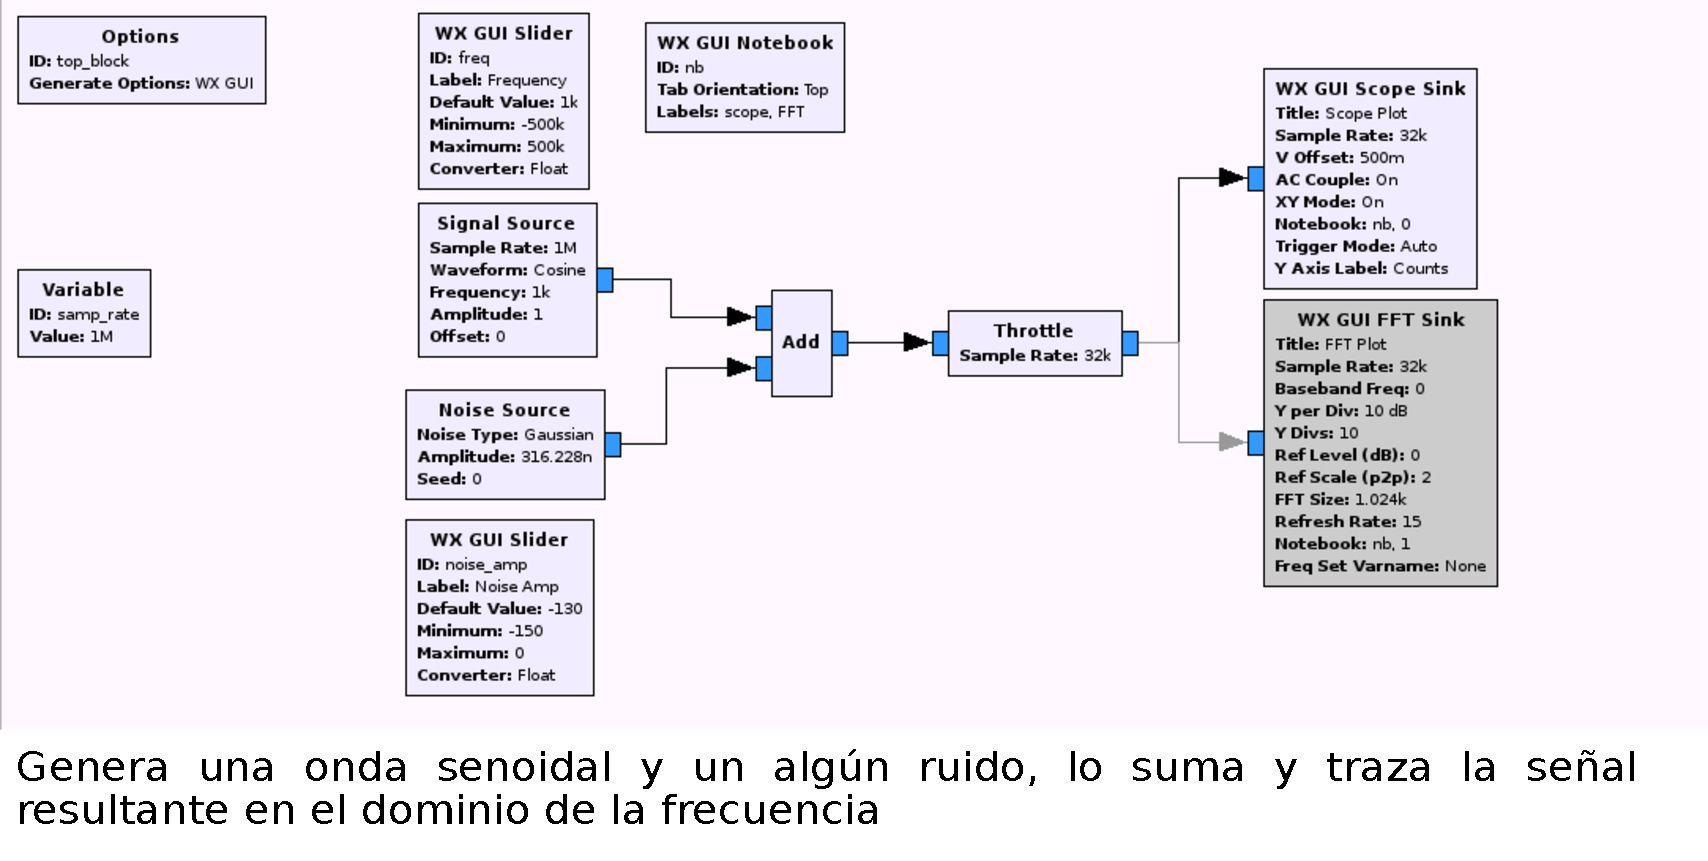
\includegraphics[width=\textwidth]{lab2/pdf/lab201.pdf}
\end{figure}
\end{frame}

\begin{frame}{Osciloscopio y FFT}
\begin{figure}[H]
\centering
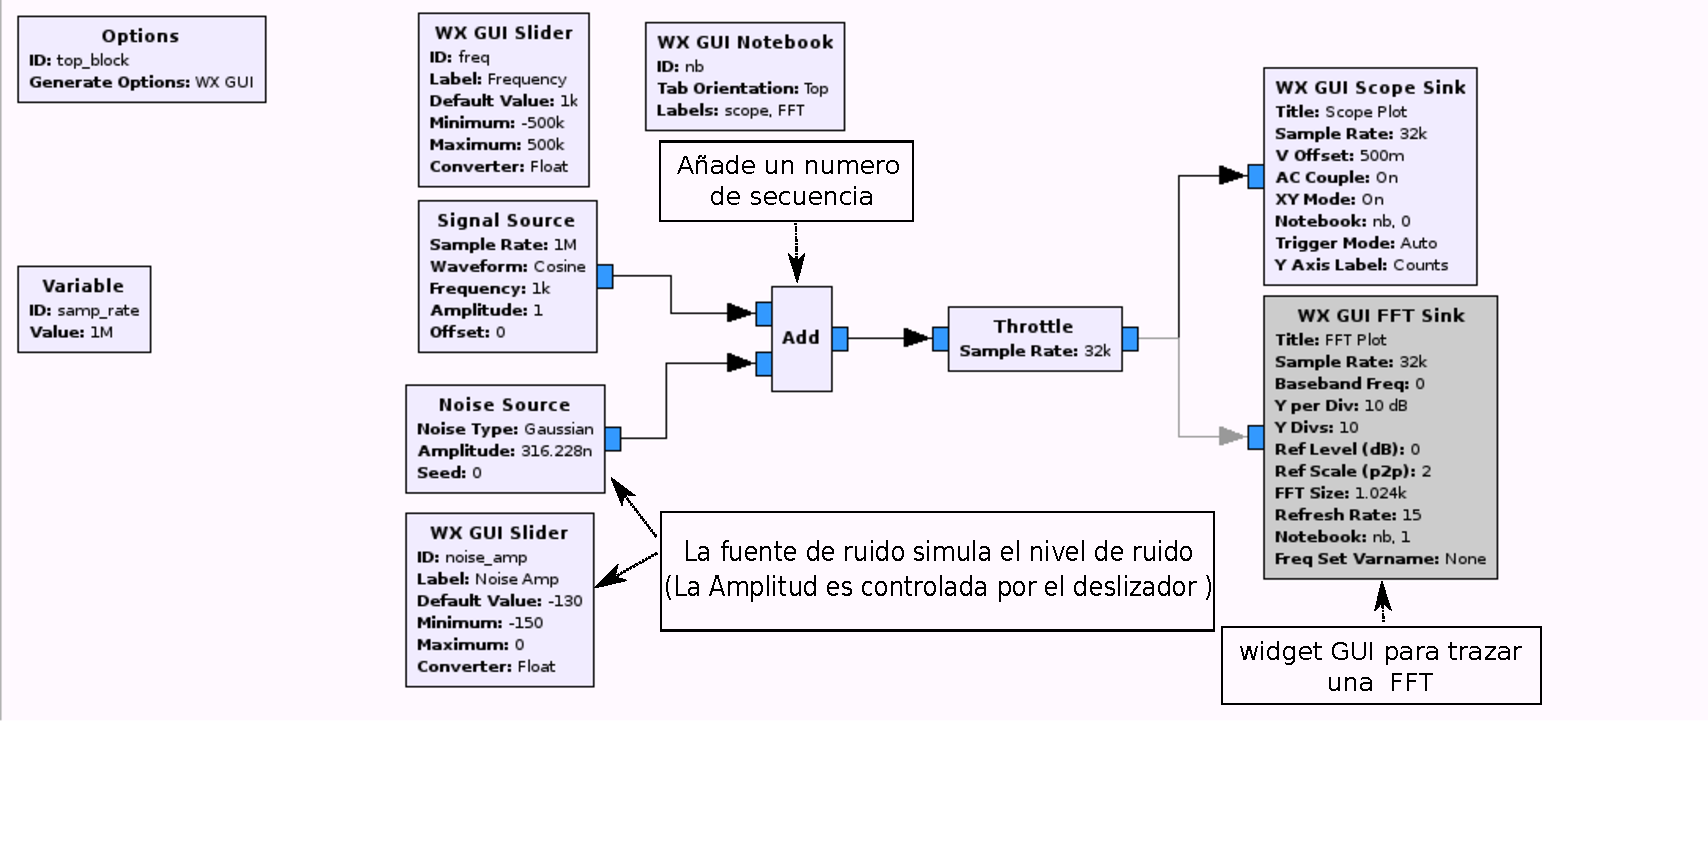
\includegraphics[width=\textwidth]{lab2/pdf/lab202.pdf}
\end{figure}
\end{frame}

\begin{frame}{Osciloscopio y FFT\index{Noise Source}}
\begin{figure}[H]
\centering
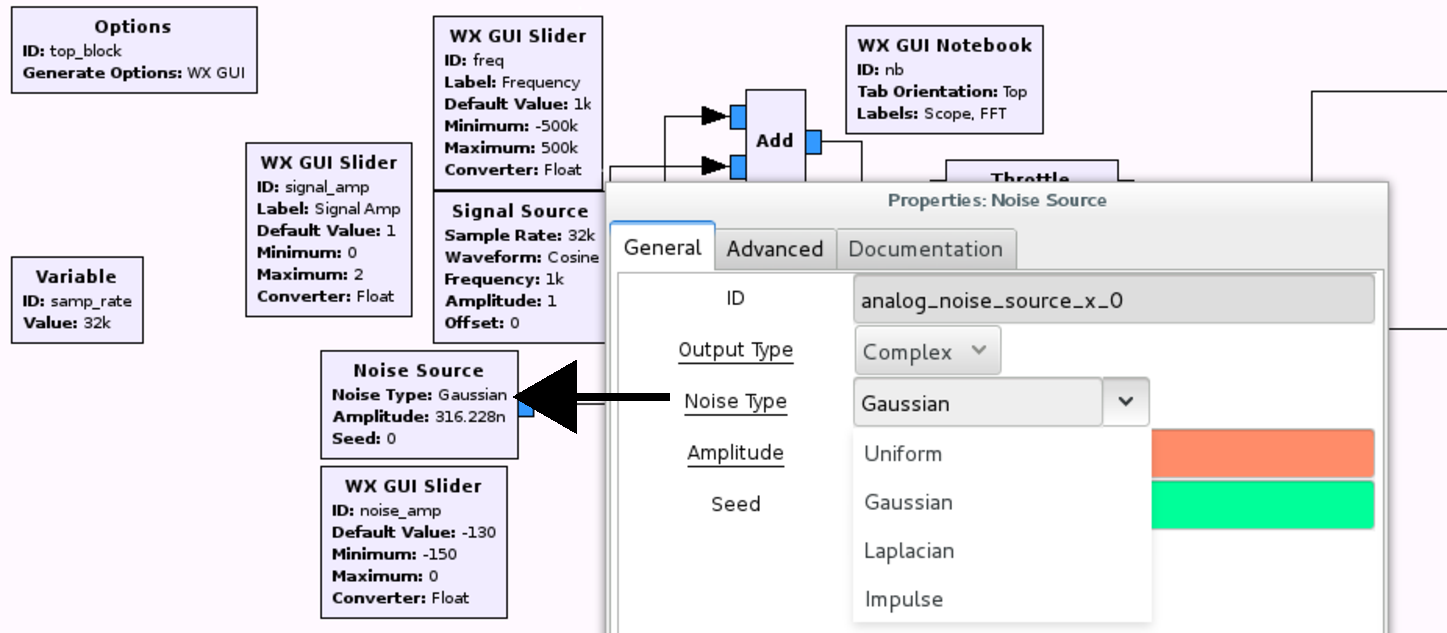
\includegraphics[width=\textwidth]{lab2/pdf/lab203.pdf}
\end{figure}
\end{frame}

\begin{frame}{Osciloscopio y FFT\index{Noise Source}}
\begin{figure}[H]
\centering
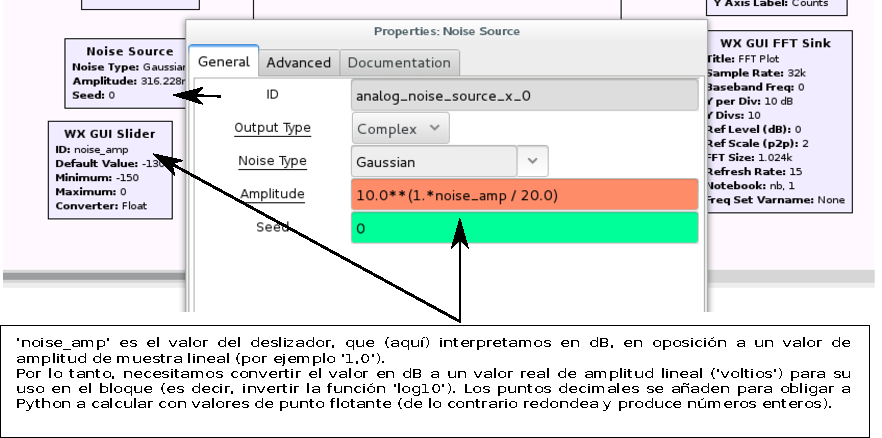
\includegraphics[width=\textwidth]{lab2/pdf/lab204.pdf}
\end{figure}
\end{frame}

\begin{frame}{Osciloscopio y FFT\index{Add}}
\begin{figure}[H]
\centering
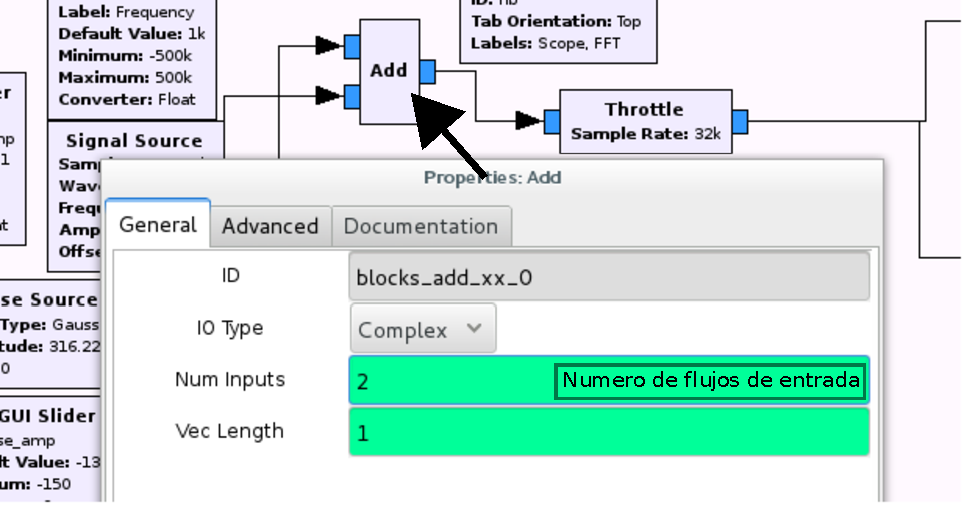
\includegraphics[width=\textwidth]{lab2/pdf/lab205.pdf}
\end{figure}
\end{frame}

\begin{frame}{Osciloscopio y FFT}
\begin{figure}[H]
\centering
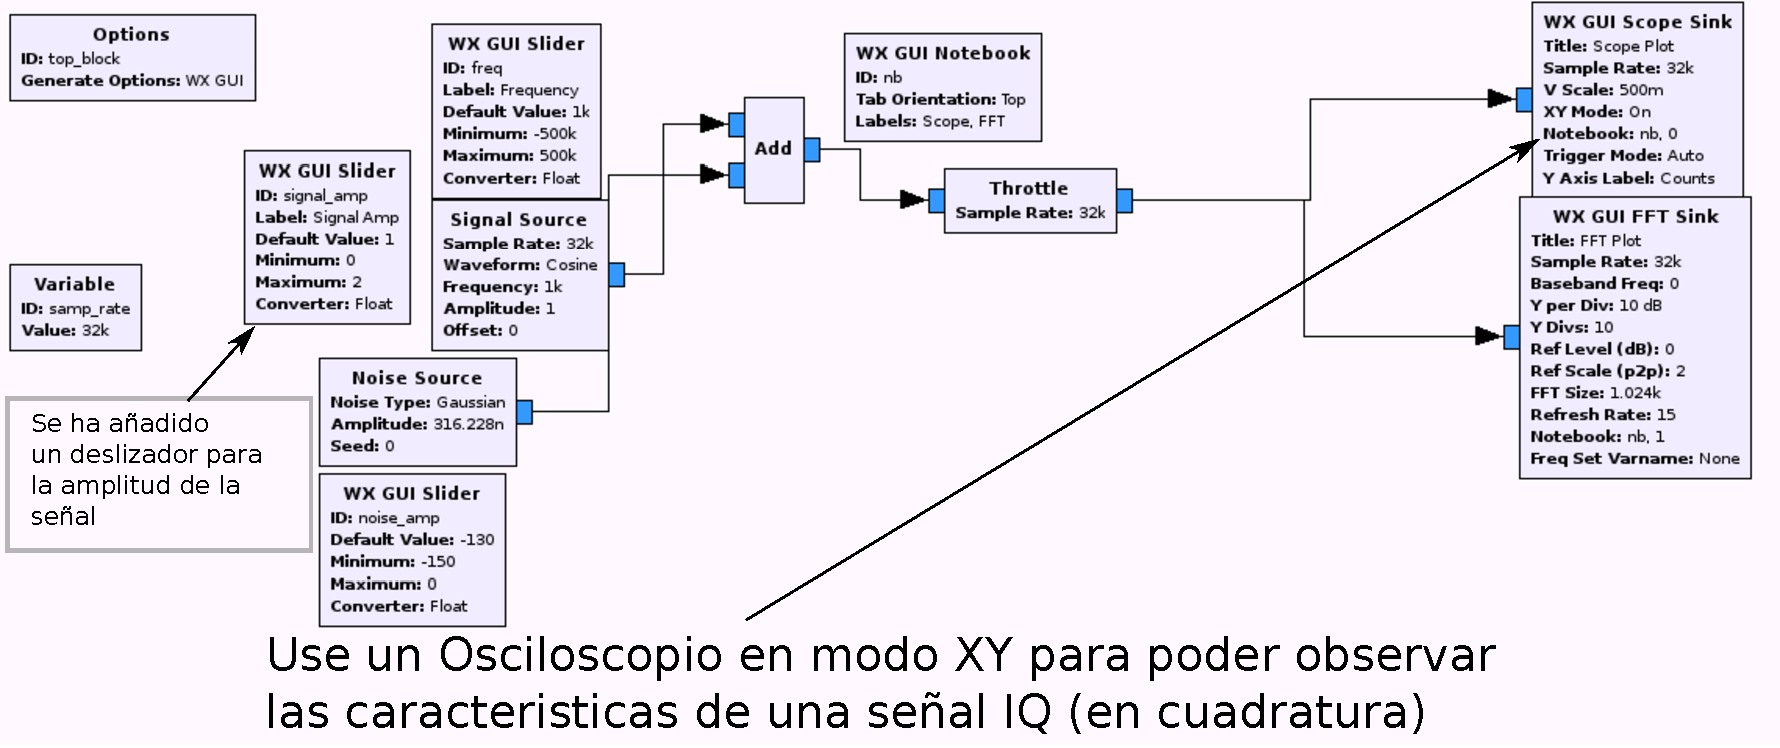
\includegraphics[width=\textwidth]{lab2/pdf/lab206.pdf}
\end{figure}
\end{frame}

\begin{frame}{Osciloscopio y FFT\index{WX GUI Notebook}}
\begin{figure}[H]
\centering
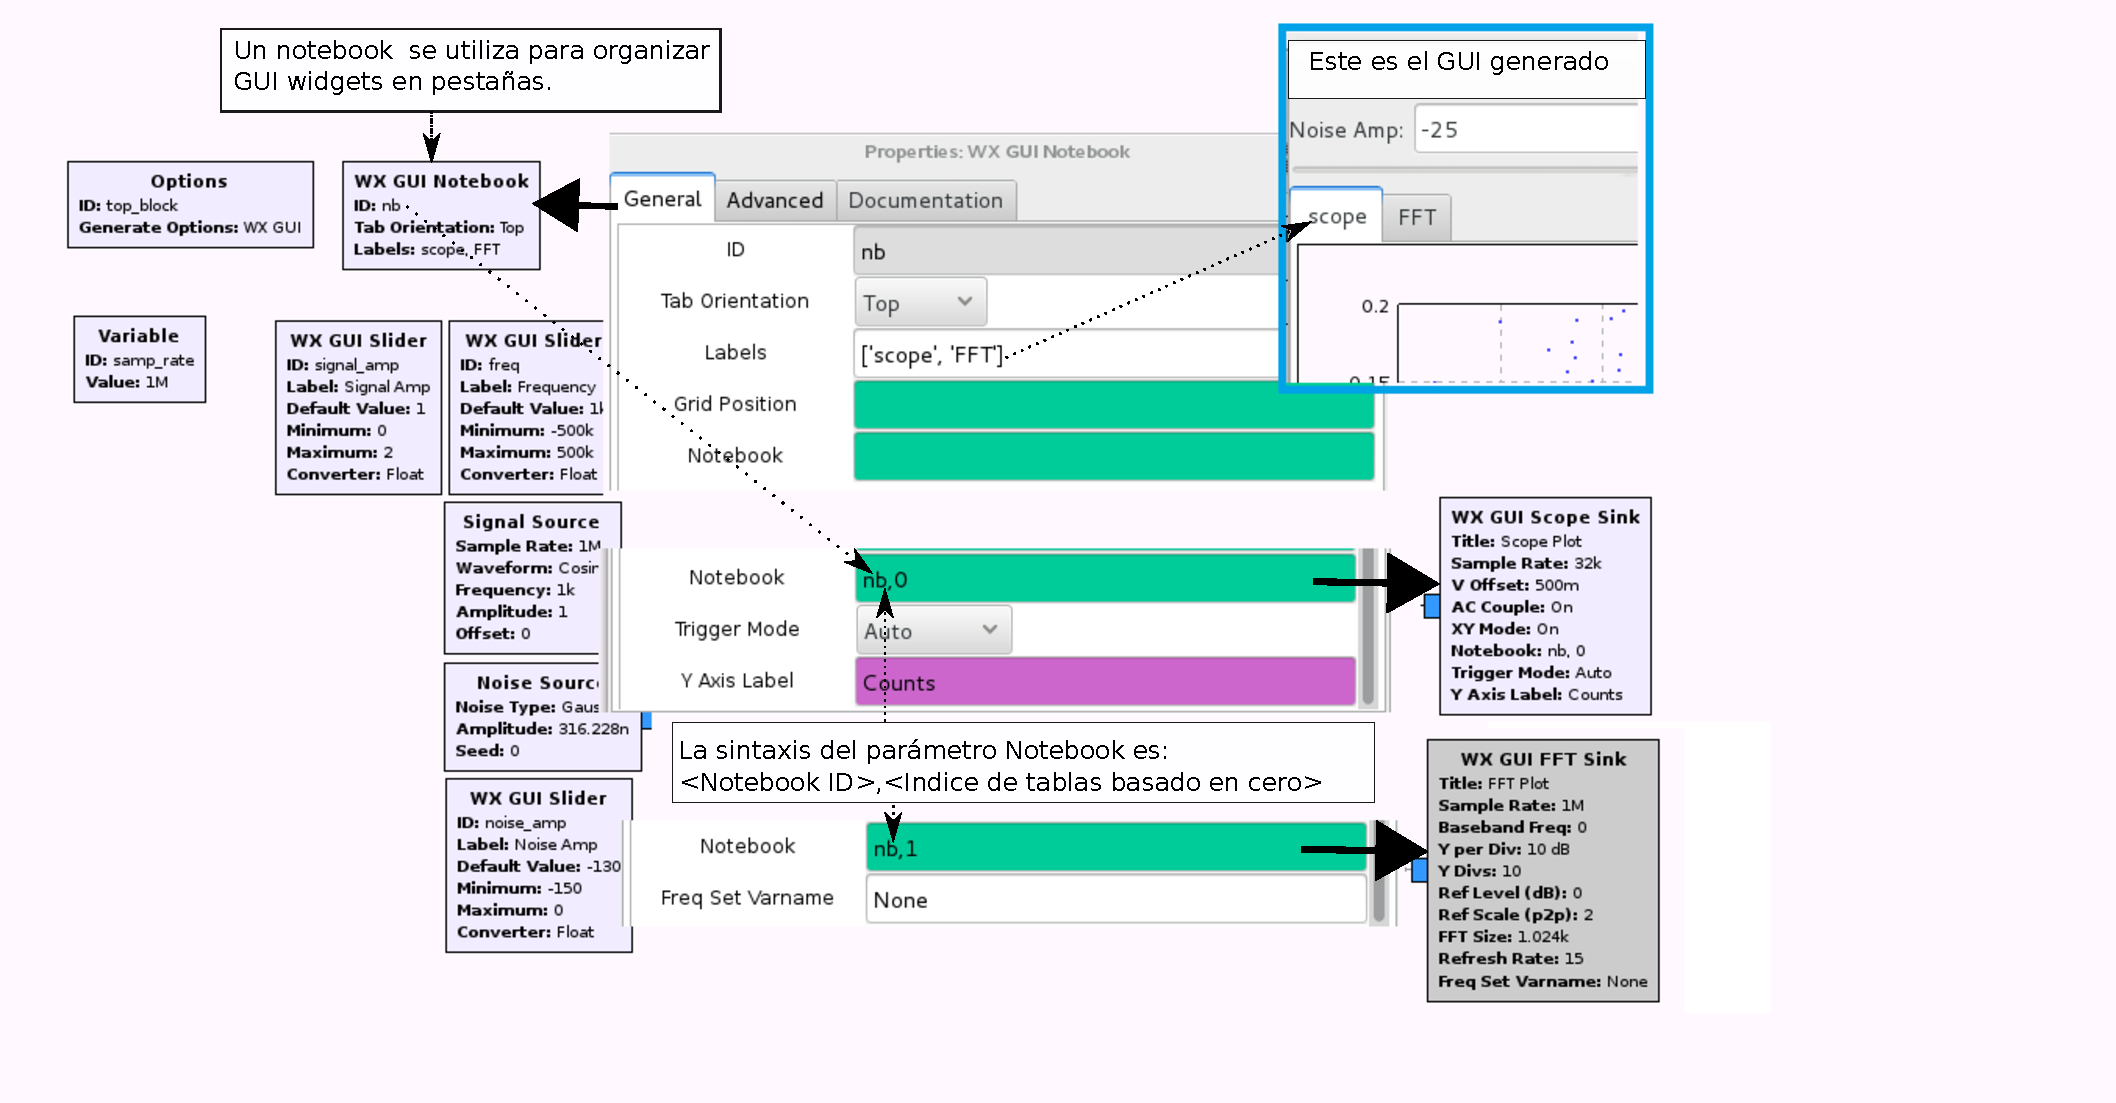
\includegraphics[width=\textwidth]{lab2/pdf/lab207.pdf}
\end{figure}
\end{frame}

\begin{frame}{Osciloscopio y FFT\index{WX GUI FFT Sink}}
\begin{figure}[H]
\centering
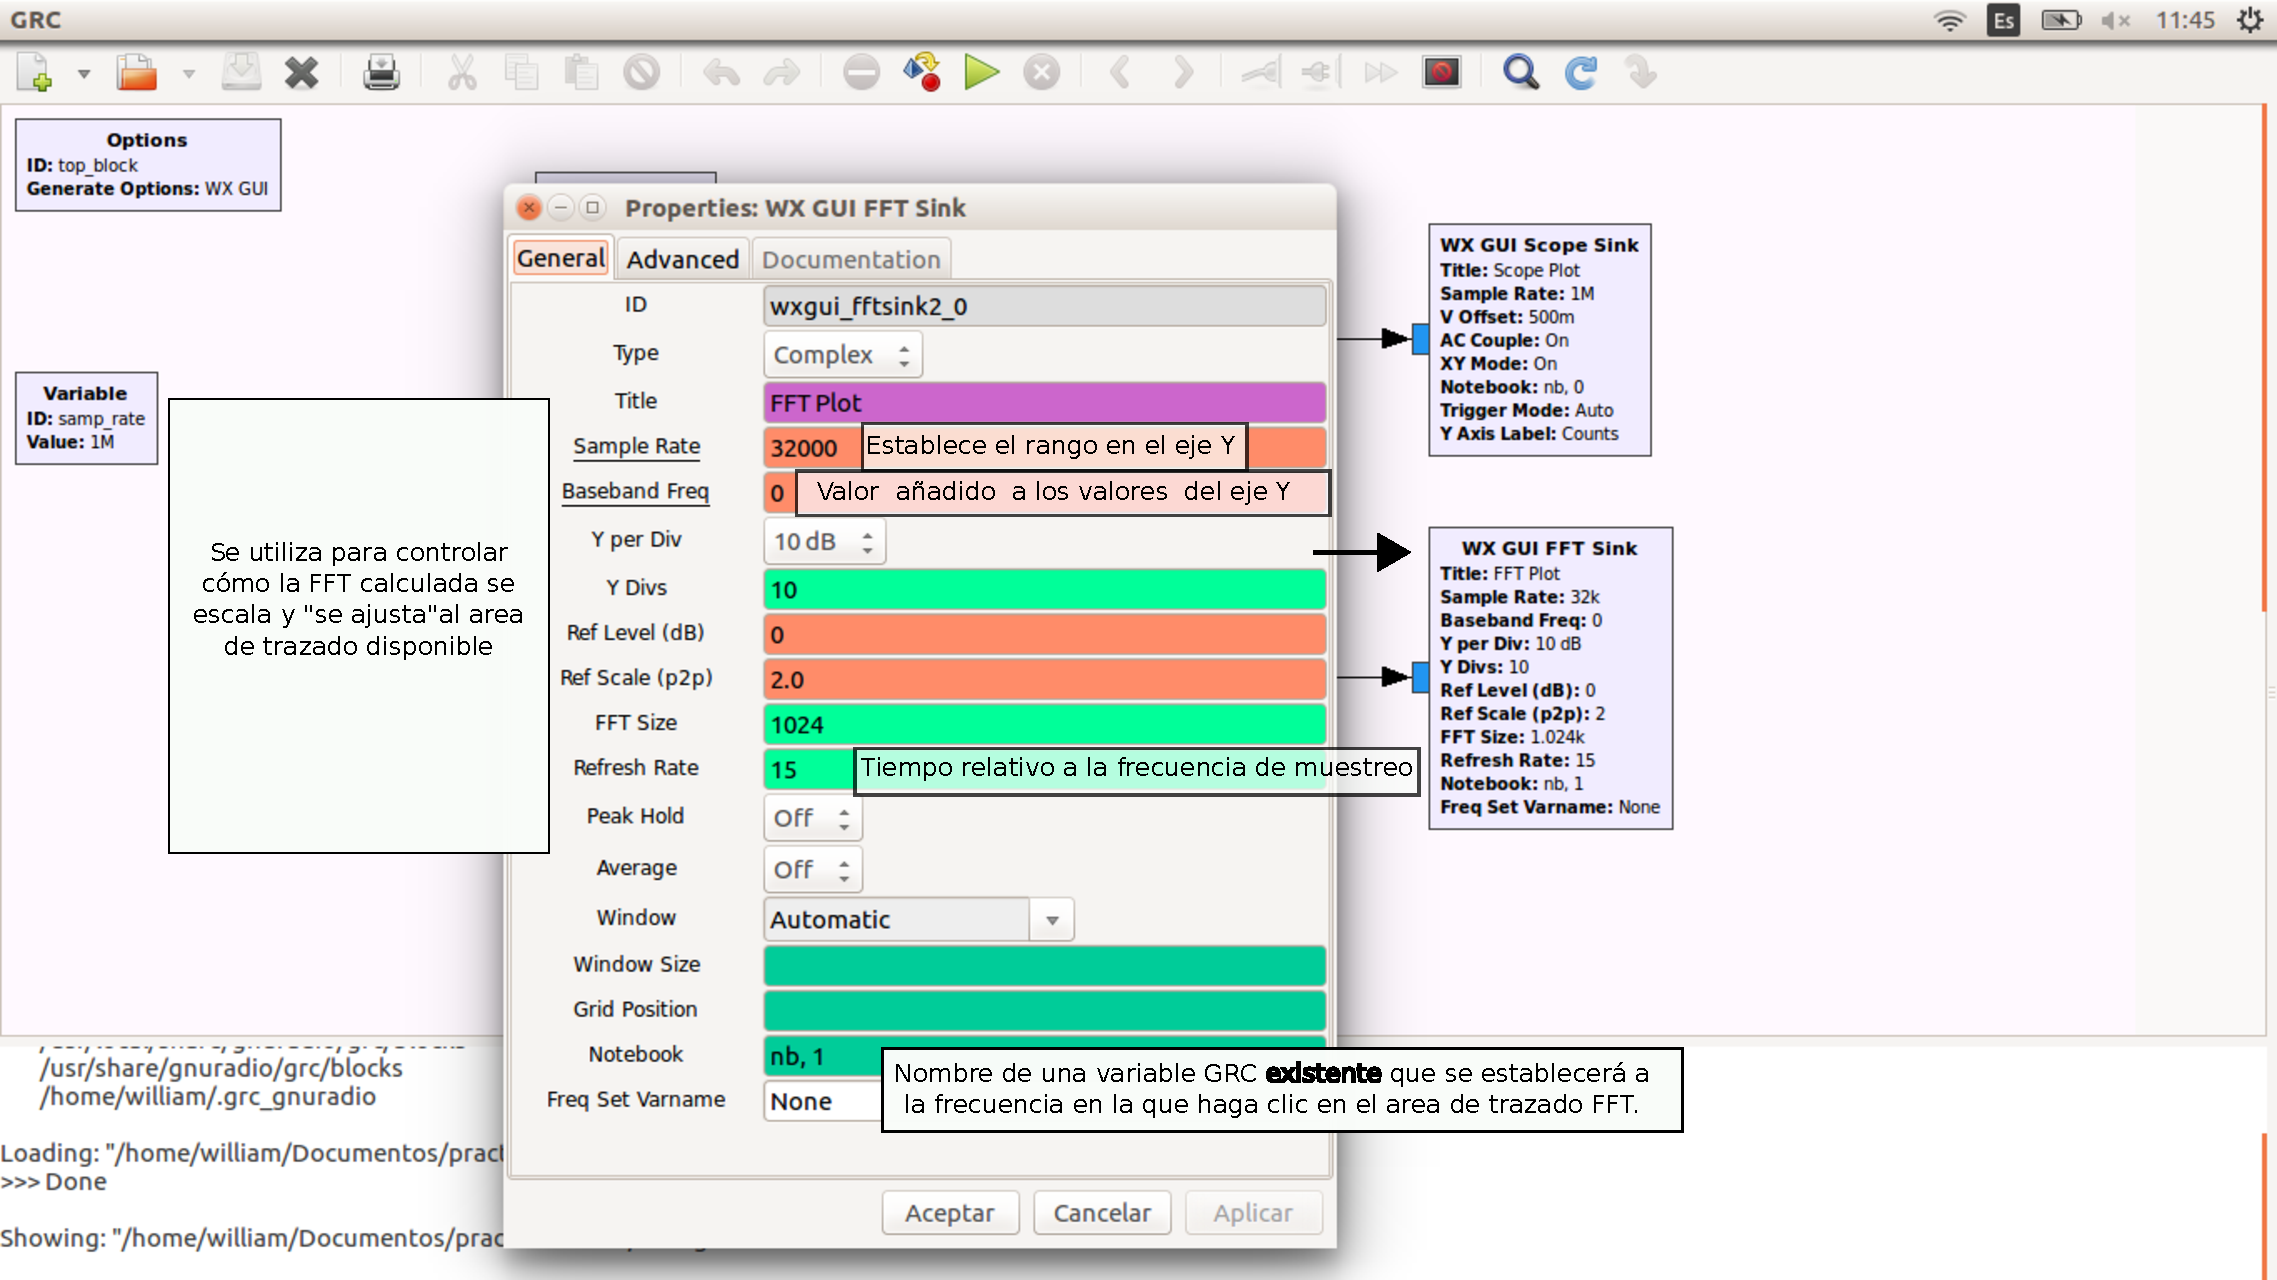
\includegraphics[width=\textwidth]{lab2/pdf/lab208.pdf}
\end{figure}
\end{frame}

\begin{frame}{Osciloscopio y FFT\index{WX GUI FFT Sink}}
\begin{figure}[H]
\centering
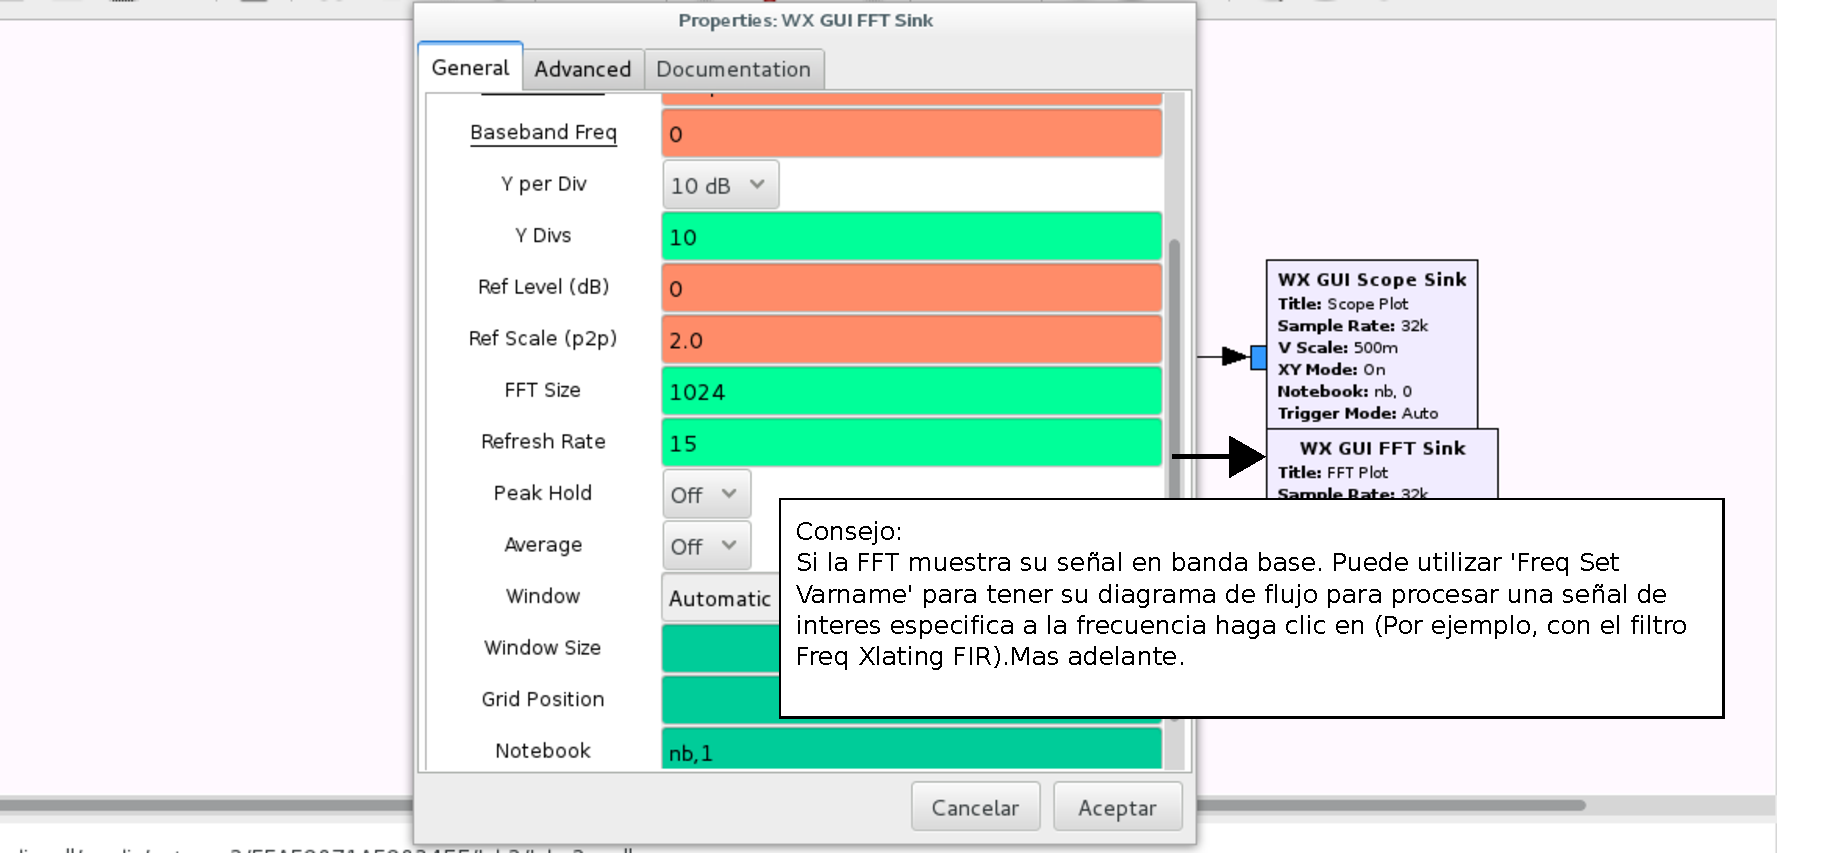
\includegraphics[width=\textwidth]{lab2/pdf/lab209.pdf}
\end{figure}
\end{frame}

\begin{frame}{Osciloscopio y FFT}
\begin{figure}[H]
\centering
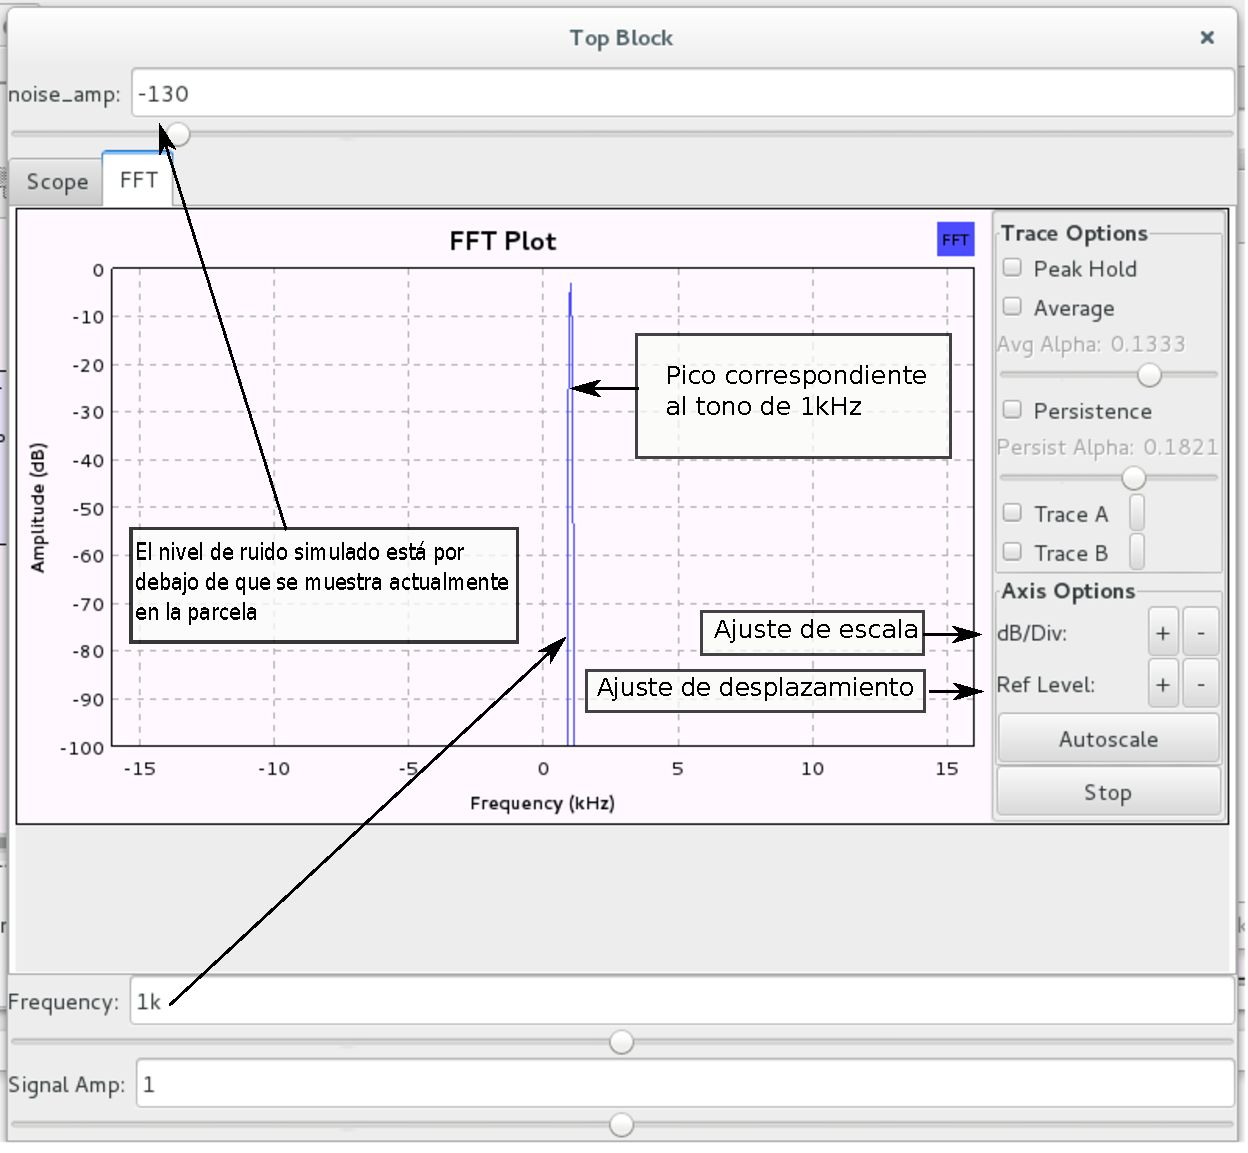
\includegraphics[width=0.9\textwidth, height=0.55\textwidth]{lab2/pdf/lab210.pdf}
\end{figure}
\end{frame}

\begin{frame}{Osciloscopio y FFT}
\begin{figure}[H]
\centering
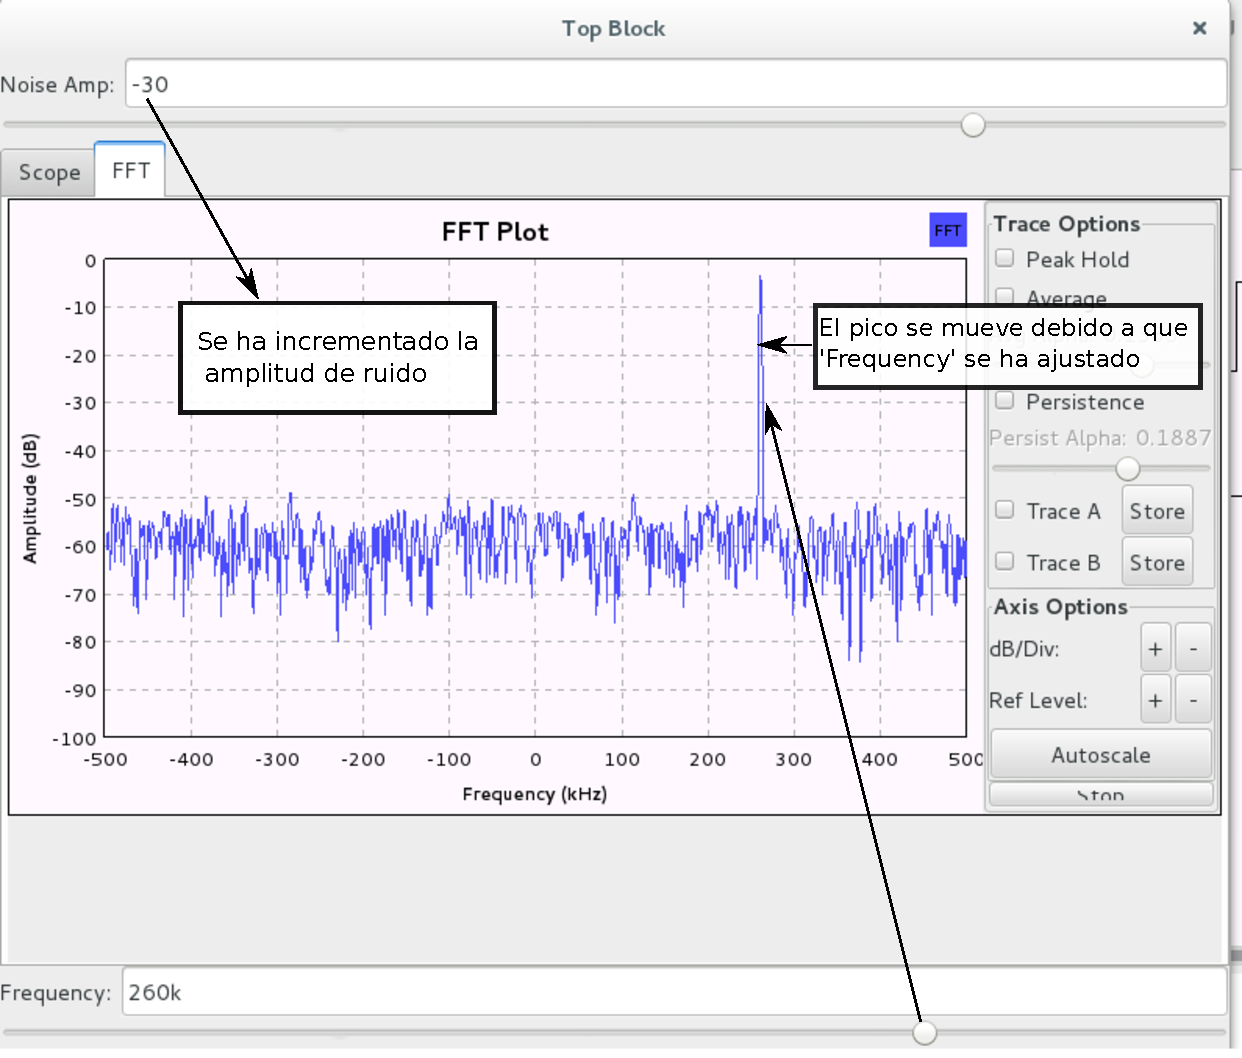
\includegraphics[width=\textwidth, height=0.55\textwidth]{lab2/pdf/lab211.pdf}
\end{figure}
\end{frame}

\begin{frame}{Osciloscopio y FFT}
\begin{figure}[H]
\centering
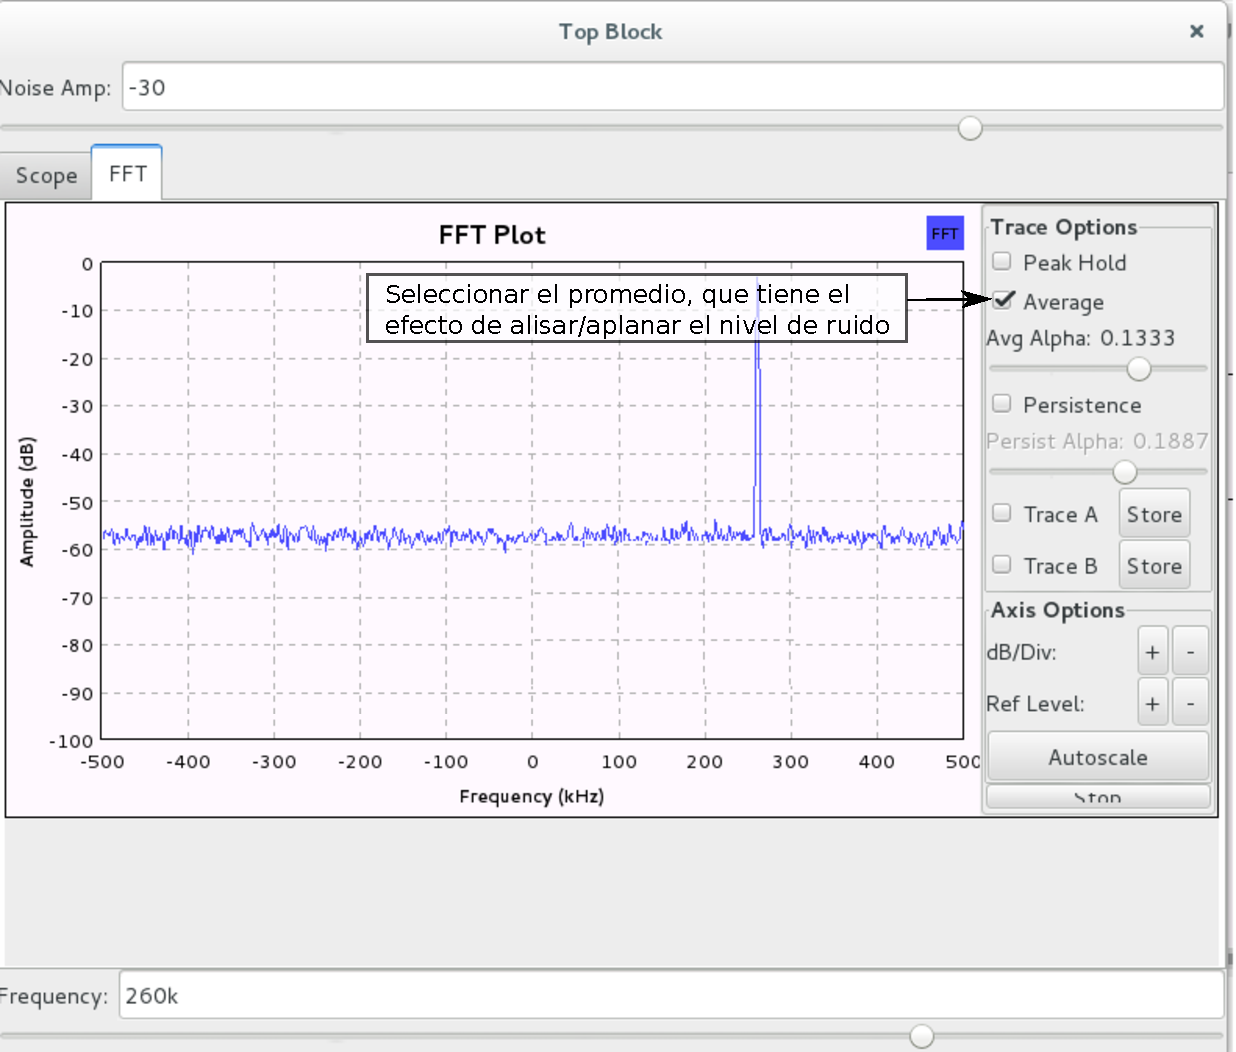
\includegraphics[width=\textwidth, height=0.58\textwidth]{lab2/pdf/lab212.pdf}
\end{figure}
\end{frame}

\begin{frame}{Osciloscopio y FFT}
\begin{figure}[H]
\centering
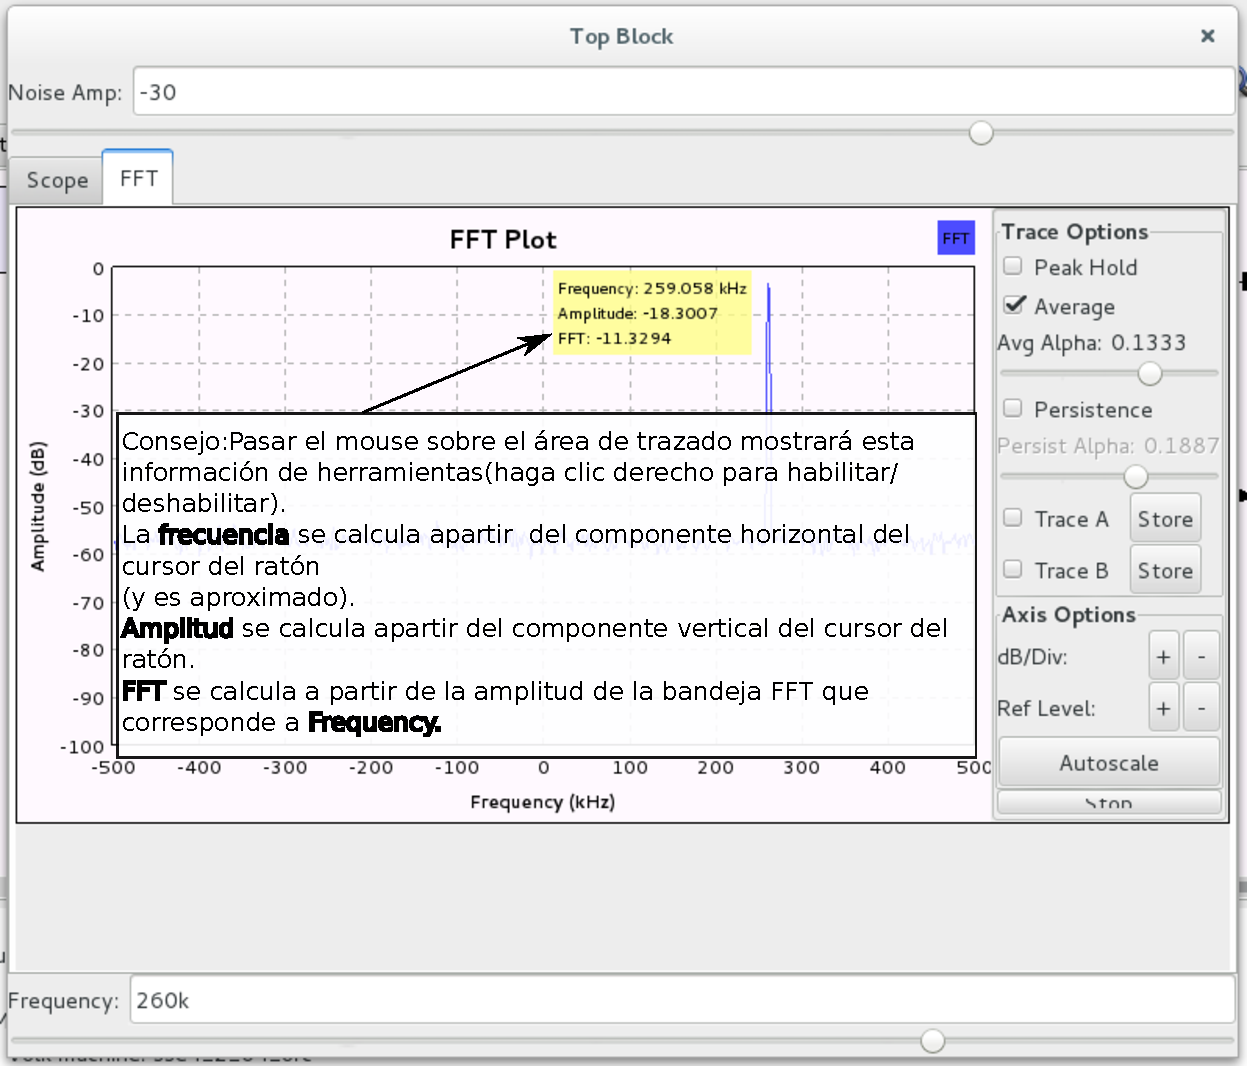
\includegraphics[width=\textwidth, height=0.58\textwidth]{lab2/pdf/lab213.pdf}
\end{figure}
\end{frame}

\begin{frame}{Osciloscopio y FFT}
\begin{figure}[H]
\centering
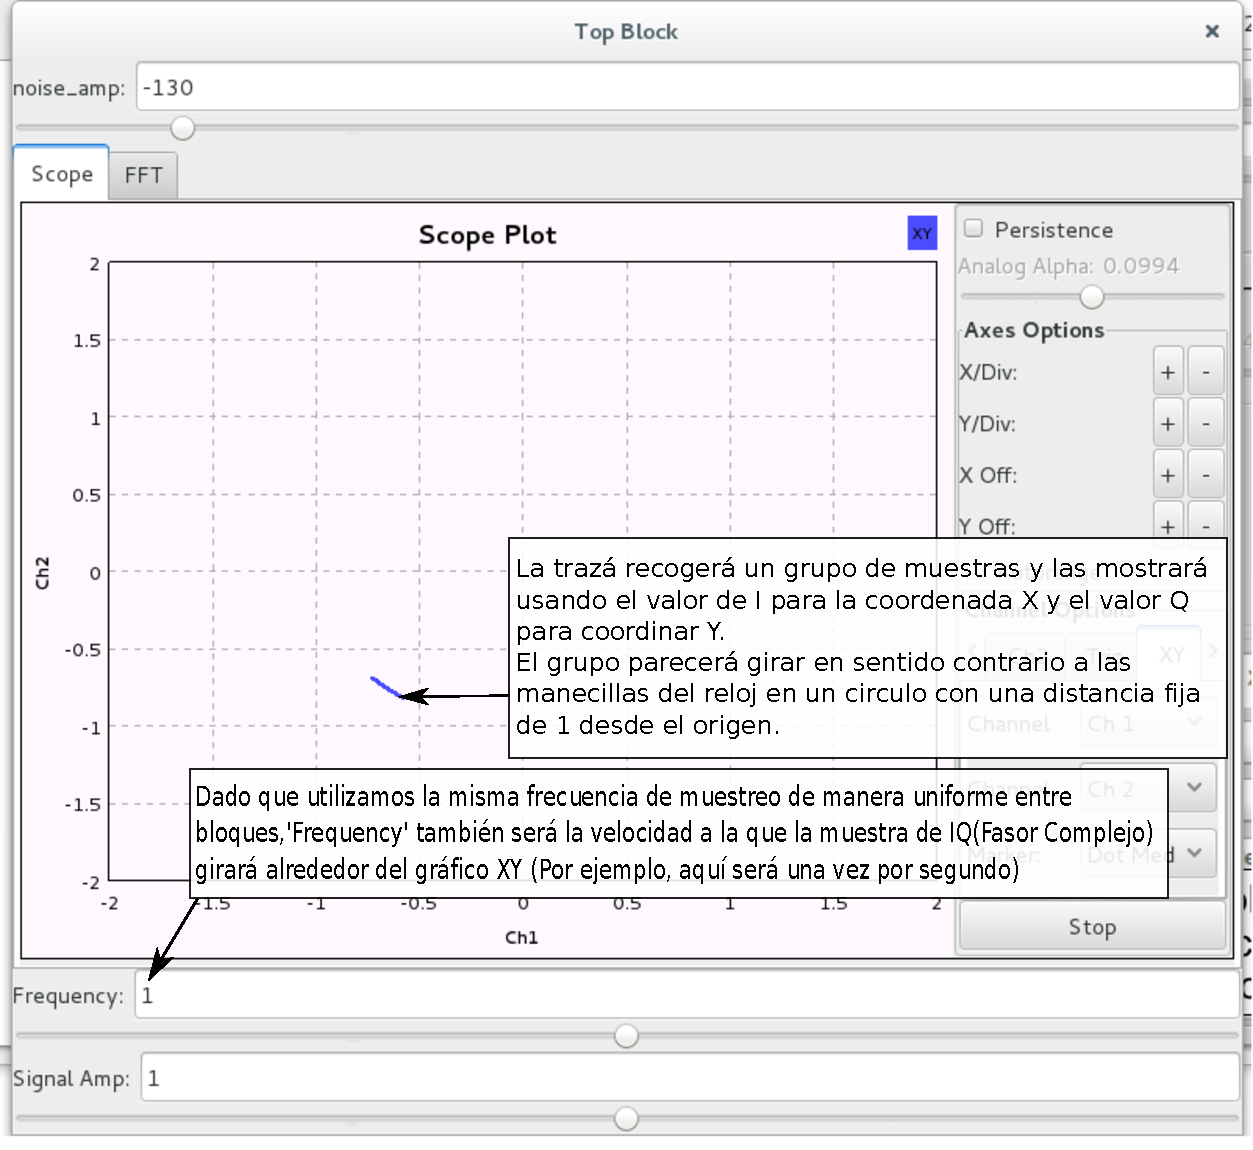
\includegraphics[width=\textwidth, height=0.58\textwidth]{lab2/pdf/lab214.pdf}
\end{figure}
\end{frame}

\begin{frame}{Osciloscopio y FFT}
\begin{figure}[H]
\centering
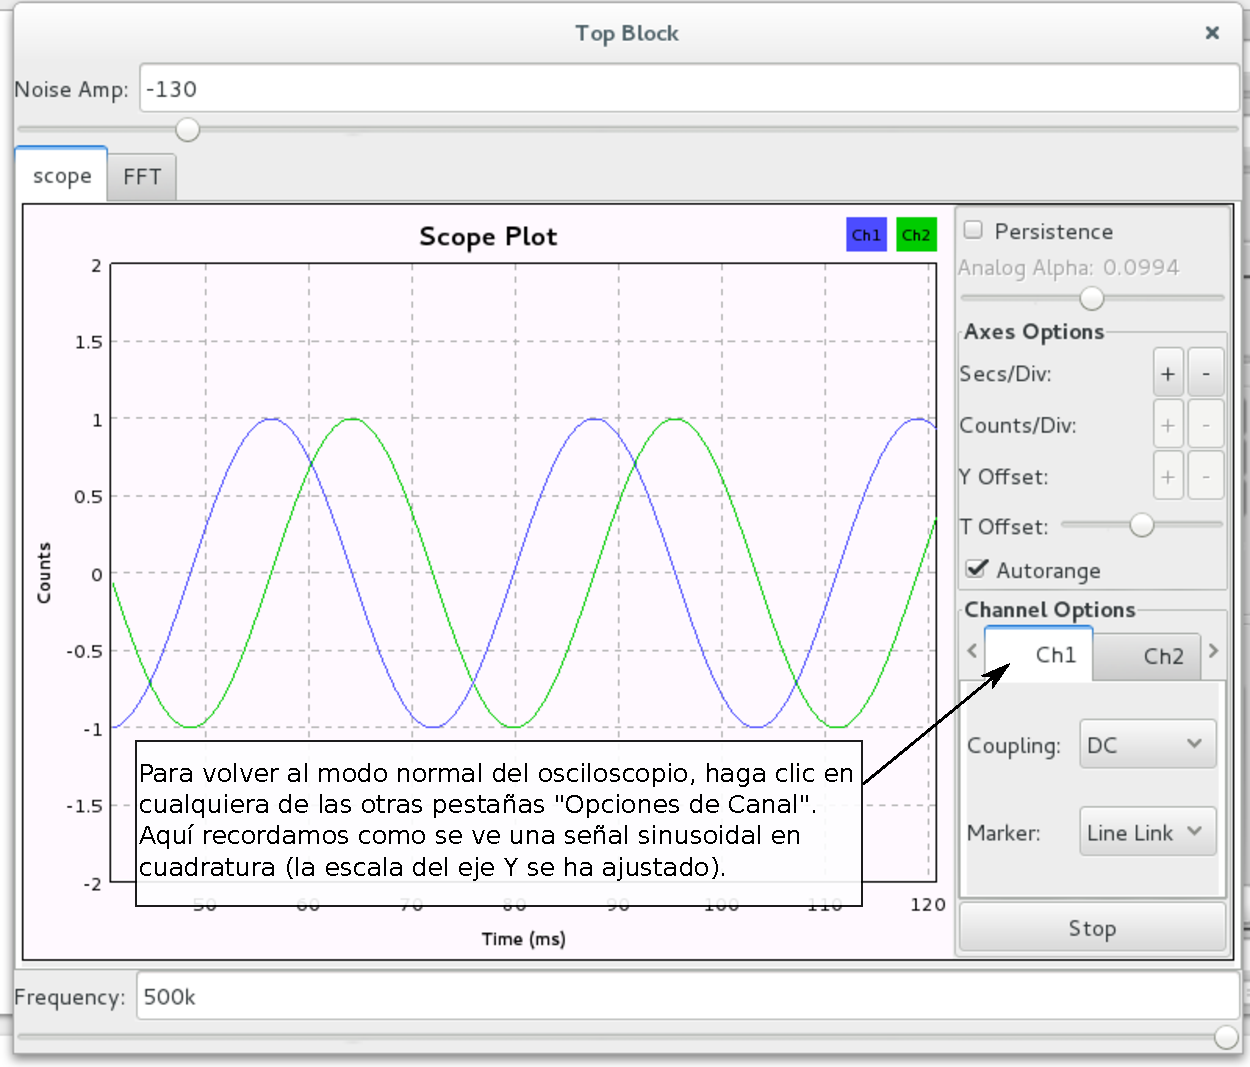
\includegraphics[width=\textwidth, height=0.58\textwidth]{lab2/pdf/lab215.pdf}
\end{figure}
\end{frame}

\begin{frame}{Osciloscopio y FFT}
\begin{figure}[H]
\centering
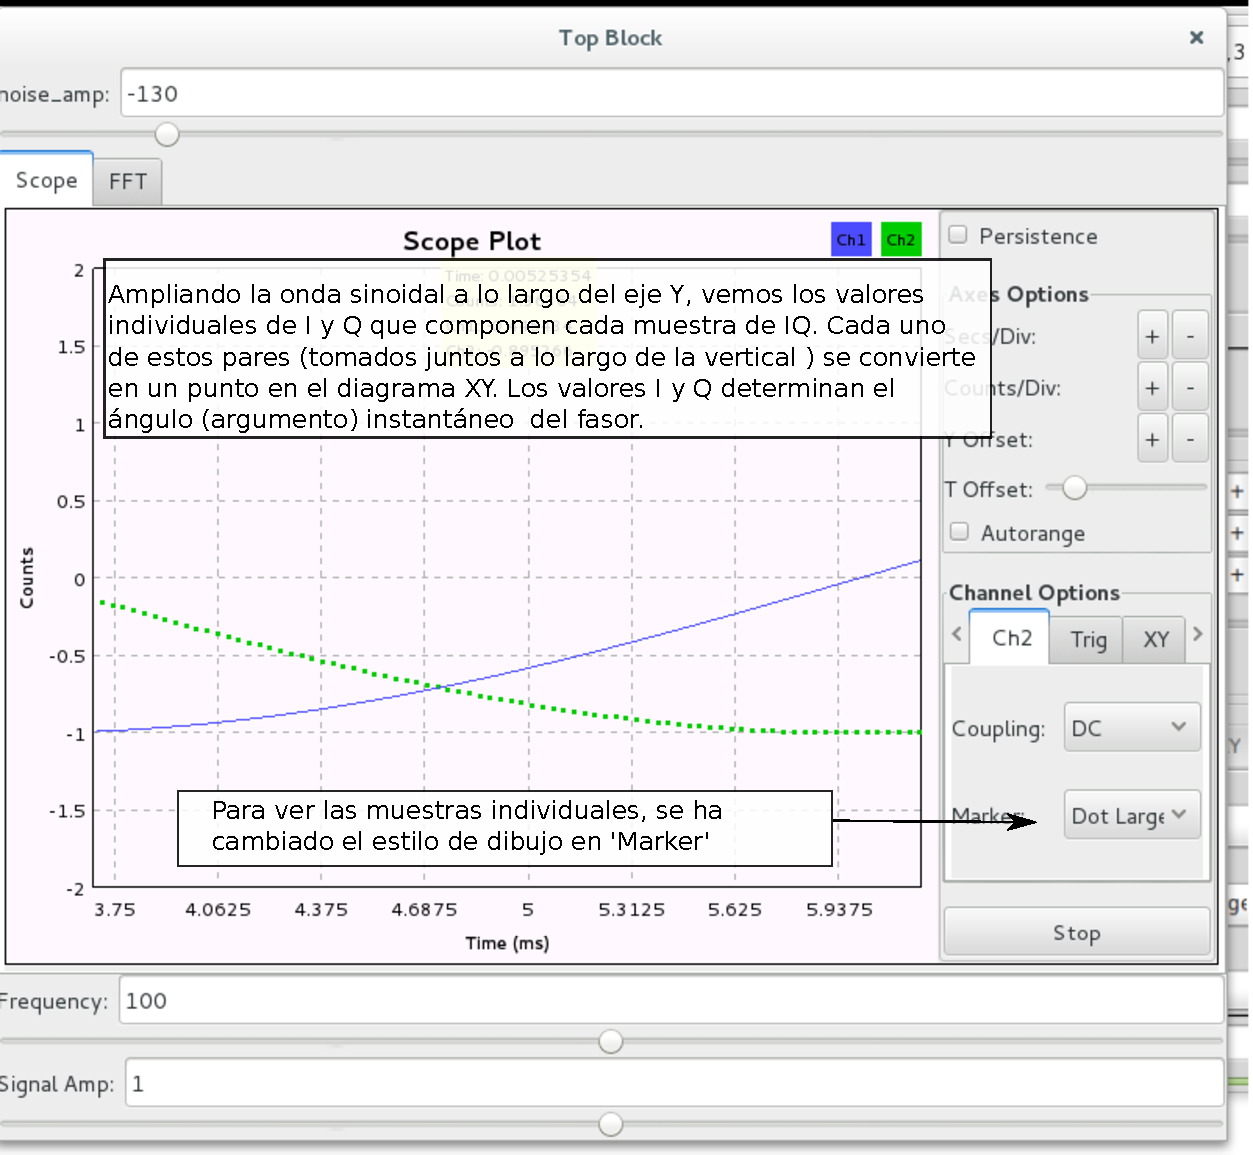
\includegraphics[width=\textwidth, height=0.58\textwidth]{lab2/pdf/lab216.pdf}
\end{figure}
\end{frame}

\begin{frame}{Osciloscopio y FFT}
\begin{figure}[H]
\centering
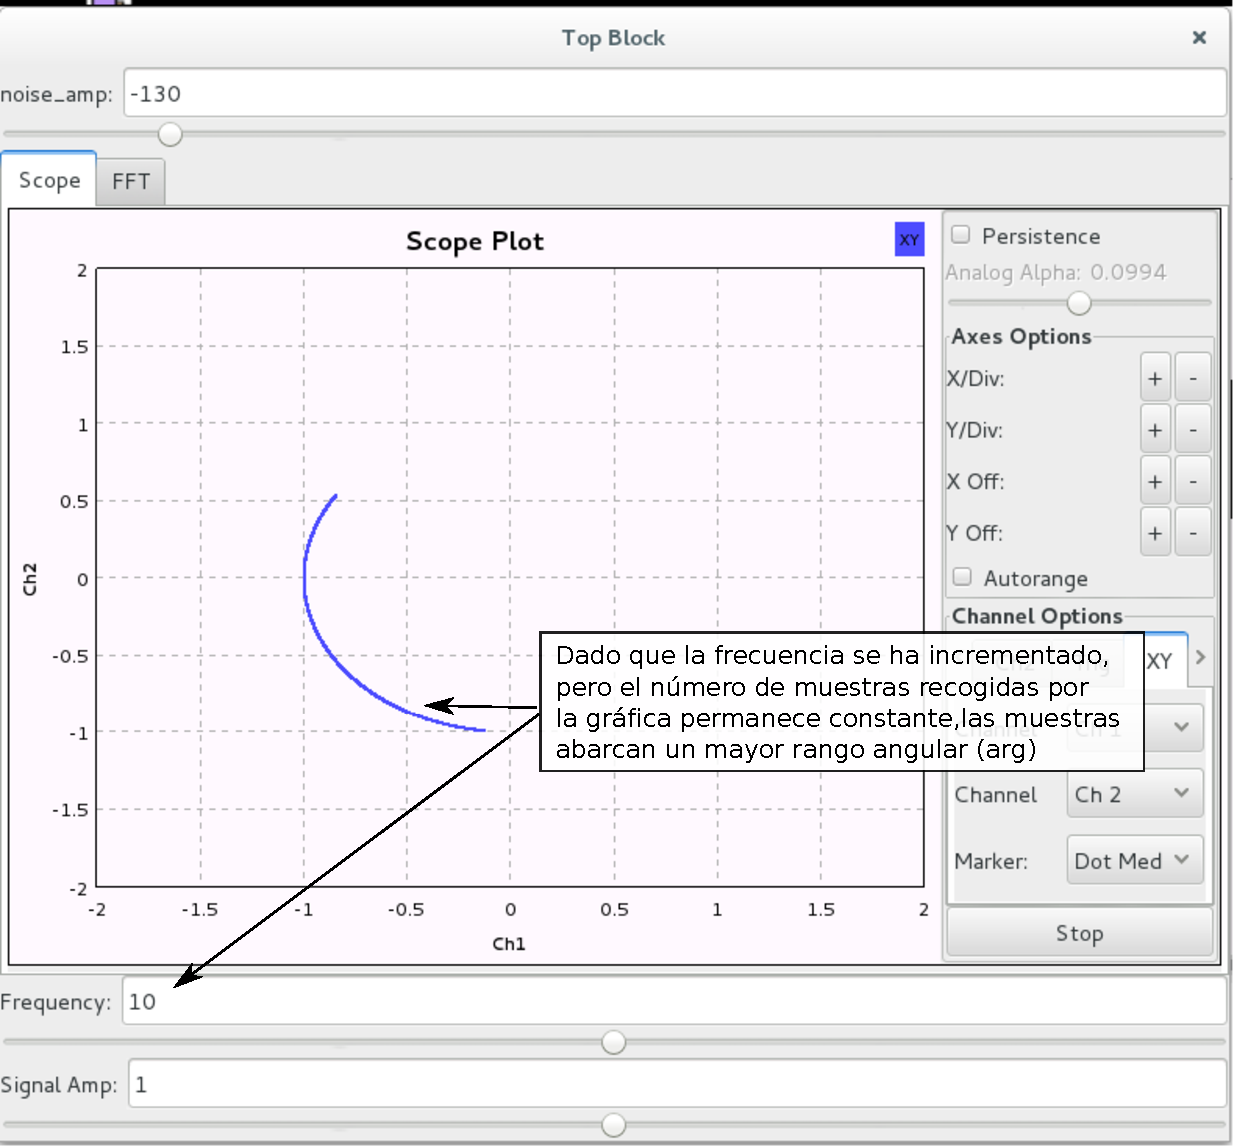
\includegraphics[width=\textwidth, height=0.58\textwidth]{lab2/pdf/lab217.pdf}
\end{figure}
\end{frame}

\begin{frame}{Osciloscopio y FFT}
\begin{figure}[H]
\centering
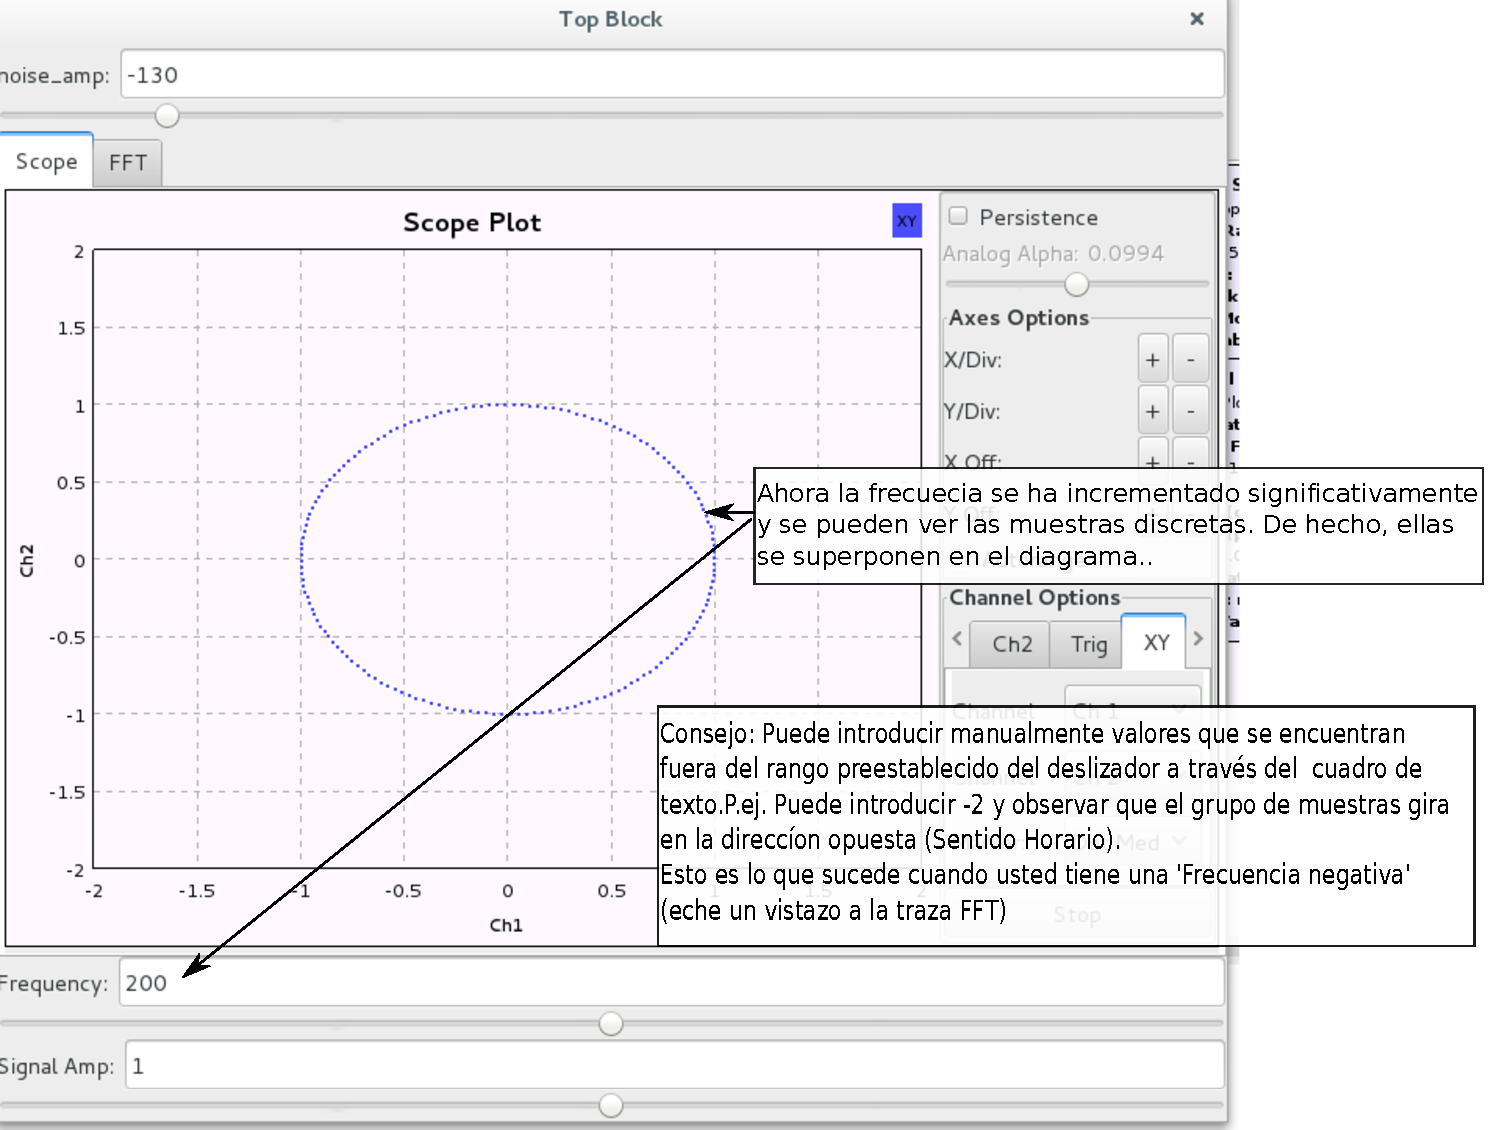
\includegraphics[width=\textwidth, height=0.58\textwidth]{lab2/pdf/lab218.pdf}
\end{figure}
\end{frame}

\begin{frame}{Osciloscopio y FFT}
\begin{figure}[H]
\centering
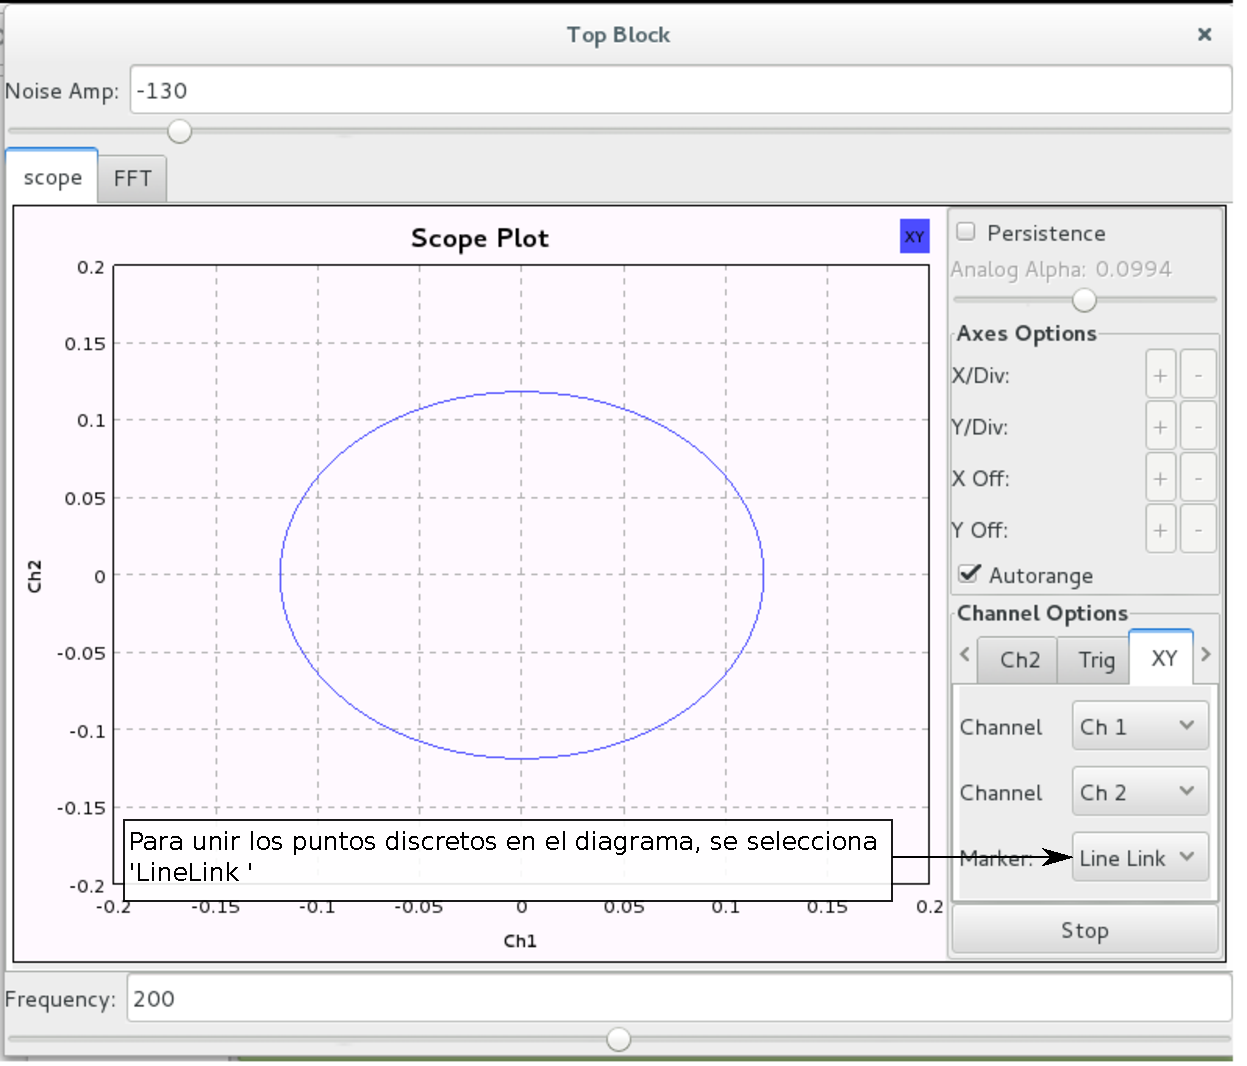
\includegraphics[width=\textwidth, height=0.58\textwidth]{lab2/pdf/lab219.pdf}
\end{figure}
\end{frame}

\begin{frame}{Osciloscopio y FFT}
\begin{figure}[H]
\centering
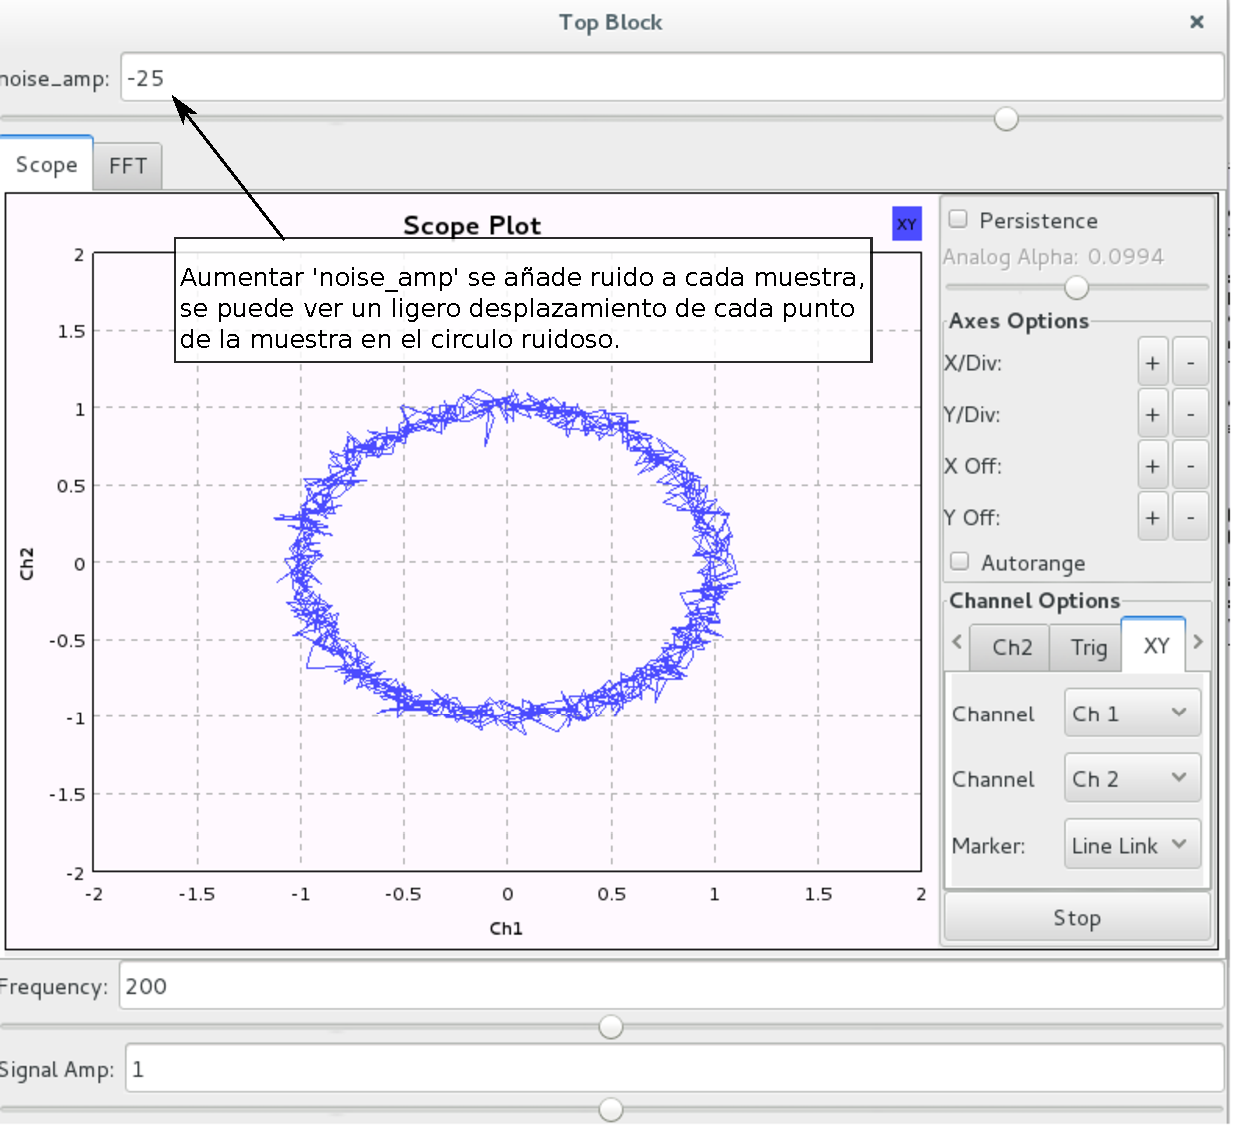
\includegraphics[width=\textwidth, height=0.58\textwidth]{lab2/pdf/lab220.pdf}
\end{figure}
\end{frame}